% Pipeline figure for the Semantic Coverage metric, in the style of
% paper/system_fig/system_overview.tex.
%   Archive images --> VLM captions --> caption text embedding --> greedy
%   farthest-point sampling + k-covering radius over caption embeddings
%   (Semantic Coverage score).
% Assets (cap_thumb_*.png, semantic_scatter.png, _semantic_meta.tex) built by
% tools/build_metric_fig_assets.py.  Compile: pdflatex semantic_novelty.tex
\documentclass[border=8pt, varwidth=false]{standalone}
% Shared TikZ styling for the eval-metric pipeline figures, matching the look of
% paper/system_fig/system_overview.tex. \input after \documentclass{standalone}.
\usepackage{tikz}
\usetikzlibrary{positioning,shapes.geometric,arrows.meta,calc,fit,backgrounds,fadings}
\usepackage{graphicx}
\usepackage{amsmath,amssymb}
\usepackage{xcolor}
\usepackage[T1]{fontenc}

\tikzset{
  >=Stealth,
  box/.style       = {draw, rounded corners=2pt, align=center,
                      inner sep=4pt, line width=0.6pt, fill=white},
  vlmbox/.style    = {box, fill=blue!5,    draw=blue!55!black},
  embbox/.style    = {box, fill=violet!7,  draw=violet!60!black},
  databox/.style   = {box, fill=black!3,   draw=black!45},
  scorebox/.style  = {box, fill=orange!12, draw=orange!75!black, line width=0.9pt},
  img/.style       = {draw=black!45, line width=0.4pt, inner sep=0, outer sep=0},
  pipe/.style      = {->, line width=0.7pt, draw=black!75},
  feed/.style      = {->, line width=0.9pt, draw=orange!75!black},
  frame/.style     = {draw=black!45, line width=0.5pt, rounded corners=4pt,
                      inner sep=10pt},
  colTitle/.style  = {font=\bfseries, anchor=south west},
}


\IfFileExists{_semantic_meta.tex}{% auto-generated by tools/build_metric_fig_assets.py
\def\captionCells{0/{A black and white line drawing of the silhouette of a sports car.}, 1/{A black and white drawing of a Stormtrooper helmet.}, 2/{A minimalist black and white line drawing of a cat looking up.}}
\def\visualScore{0.606}
\def\semanticScore{0.686}
}{%
  \def\captionCells{0/{A black and white line drawing of the silhouette of a sports car.},
    1/{A black and white drawing of a Stormtrooper helmet.},
    2/{A minimalist black and white line drawing of a cat looking up.}}%
  \def\visualScore{0.606}\def\semanticScore{0.686}}

\begin{document}
\begin{tikzpicture}[font=\footnotesize, x=1cm, y=1cm]

% ===================== SOURCE: ARCHIVE =====================
\node[frame, minimum width=4.6cm, minimum height=4.6cm, anchor=north west]
  (arch) at (0,0) {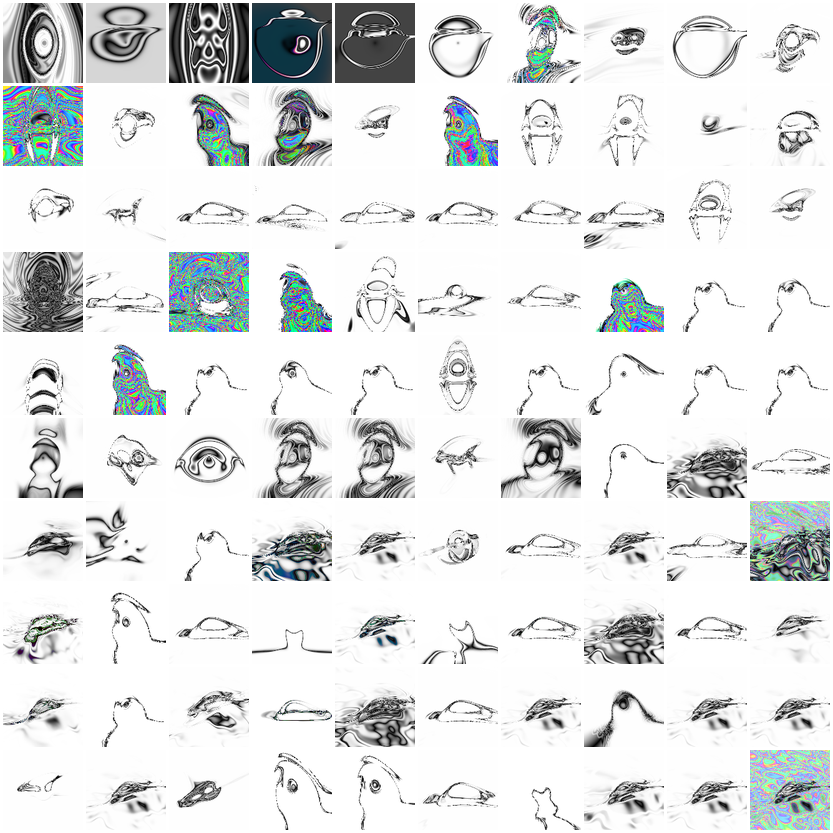
\includegraphics[width=4.0cm]{archive_grid.png}};
\node[colTitle] at (arch.north west) {Archive};

% ===================== VLM CAPTION =====================
\node[vlmbox, anchor=west, text width=2.3cm]
  (vlm) at (5.5,-2.3) {VLM caption\\ {\scriptsize gemini-2.5-pro}};
\draw[feed] (arch.east) -- (arch.east -| vlm.west);

% ===================== CAPTION EXAMPLES =====================
\node[frame, anchor=north west, minimum width=5.9cm, minimum height=4.6cm]
  (cap) at (8.7,0) {};
\node[colTitle, align=left] at (cap.north west) {Captions};
\coordinate (cgo) at ([xshift=1.0cm, yshift=-1.35cm]cap.north west);
\foreach \ic/\cp in \captionCells {%
  \node[img] (ct-\ic) at ([yshift={-\ic*1.42cm}]cgo)
    {\includegraphics[width=1.1cm]{cap_thumb_\ic.png}};
  \node[anchor=west, text width=3.55cm, font=\scriptsize, align=left, inner sep=2pt]
    at ([xshift=0.55cm]ct-\ic.east) {``\cp''};
}
\draw[feed] (vlm.east) -- (vlm.east -| cap.west);

% ===================== TEXT EMBED =====================
\node[embbox, anchor=west, text width=2.35cm]
  (emb) at (15.4,-2.3) {text\\ embedding\\ {\scriptsize gemini-embedding}};
\draw[feed] (cap.east) -- (cap.east -| emb.west);

% ===================== EMBEDDING-SPACE PANEL =====================
\node[frame, anchor=north west, minimum width=6.0cm, minimum height=6.0cm]
  (sp) at (18.9,0) {};
\node[colTitle, align=left] at (sp.north west) {Caption-embedding space};
\node[anchor=north] (scat) at ([yshift=-0.15cm]sp.north)
  {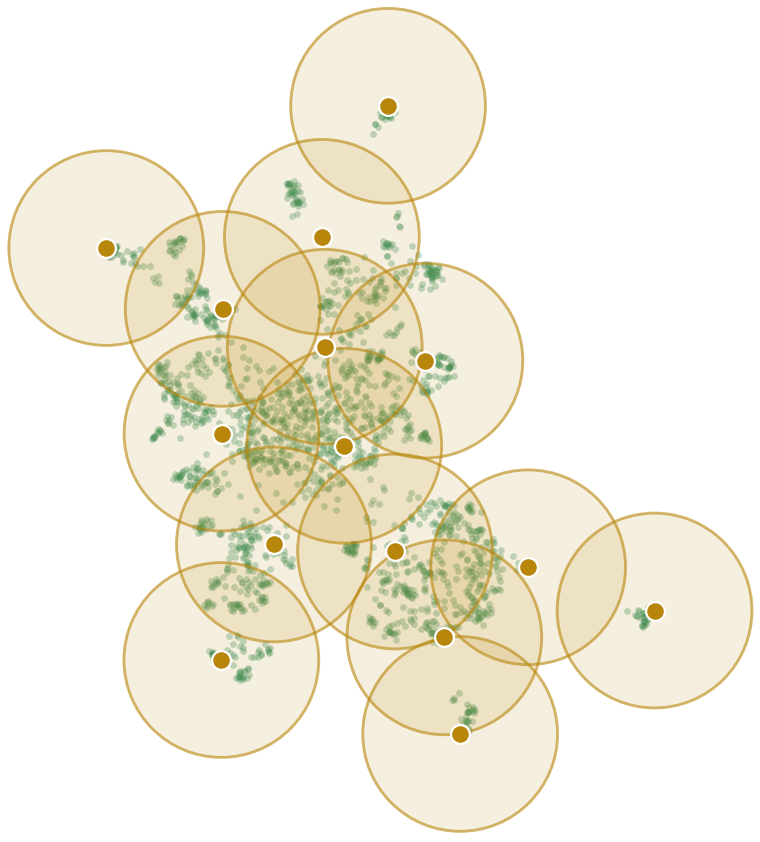
\includegraphics[width=5.0cm]{semantic_scatter.png}};
\node[anchor=south west, font=\scriptsize, align=left]
  at ([xshift=0.15cm, yshift=0.1cm]sp.south west)
  {\tikz\fill[orange!70!black] (0,0) circle (2.2pt); ~$k$ representatives (farthest-point sampling)\\
   \tikz\draw[orange!70!black, line width=0.7pt] (0,0) circle (3pt); ~equal spheres grown until all covered $\Rightarrow$ radius};
\draw[feed] (emb.east) -- node[above, align=center, font=\scriptsize]
  {farthest-point\\ sampling} (emb.east -| sp.west);

% ===================== SCORE =====================
\node[scorebox, anchor=north, align=center]
  (score) at ([yshift=-0.75cm]sp.south)
  {\textbf{Semantic Coverage} $\;=\;$ $k$-covering radius $(k=100)$
   over caption embeddings\\[1pt]
   {\scriptsize larger radius $\Rightarrow$ more semantically distinct forms}};
\draw[pipe] (sp.south) -- (sp.south |- score.north);

\end{tikzpicture}
\end{document}
